\subsection{Red neuronal Convolucional}

Las redes neuronales convolucionales tienen sus bases en el Neocognitron introducido por  Kunihiko Fukushima\cite{Fukushima_1980}. Este modelo fue mejorado por Yann LeCun\cite{Lecun_1998} al emplear un método de aprendizaje basado en la propagación hacia atrás para entrenar el sistema correctamente. En el año 2012, Dan Ciresan refino e implemento el modelo para unidades de procesamiento gráfico (GPU) consiguiendo mejores resultados\cite{Cirecsan_2011}.

Las redes neuronales convolucionales consisten en múltiples capas de filtros convolucionales de una o más dimensiones. Por lo general, después del proceso de una capa de filtro se añade una función para realizar un mapeo causal no-lineal. En la figura \ref{fig:CNN} se muestra la arquitectura de una red convolucional.

\begin{figure}[H]
    \centering
    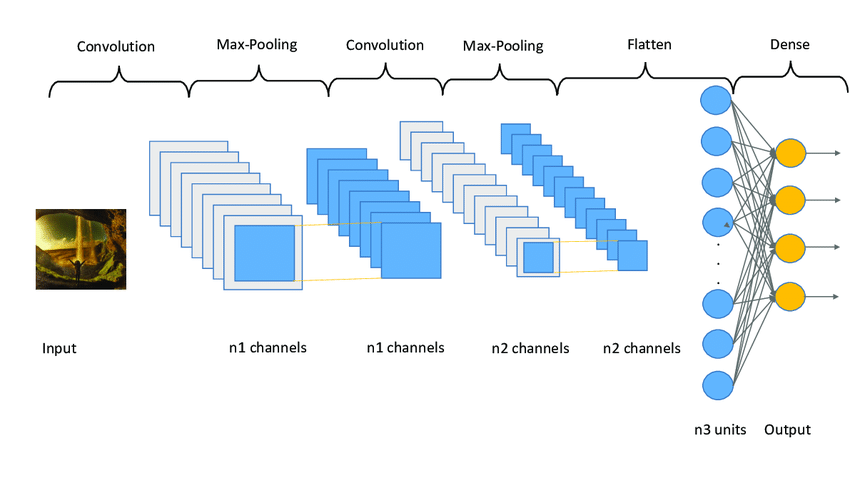
\includegraphics[width=15cm]{Graphics/convolutional.png}
    \caption{Representación visual de una red convolucional\cite{Garcia_2020}.}
    \label{fig:CNN}
\end{figure}

\subsubsection{Capa Max pooling}

La capa de Max pooling realiza una operacion que calcula el máximo valor de una submatriz. Este valor máximo es guardado en una matriz con menor dimensión que la original. En la figura \ref{fig:max_pooling} se muestra un ejemplo de como se reduce una matriz de dimensión $4x4$ a una de $2x2$.

\begin{figure}[H]
    \centering
    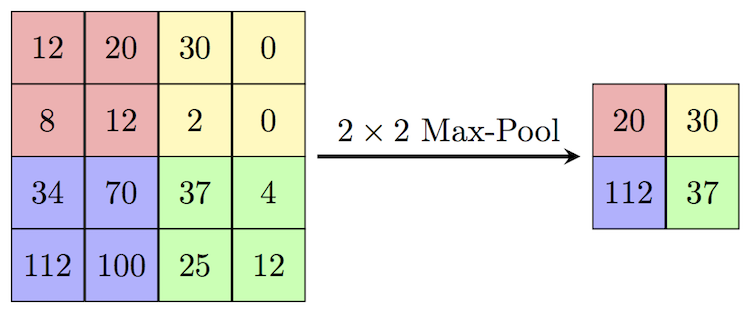
\includegraphics[width=11cm]{Graphics/max_pooling.png}
    \caption{Representación vidual de una capa con la operacion max pooling.}
    \label{fig:max_pooling}
\end{figure}